\subsection{Graphical Interface Interaction}

    A graphical web interface was chosen as solution to give users a quick
    interaction with \TVB  . The web interface is easy to access (local or
    remotely) through a web browser, it can be used by different types of
    users, including those without programming knowledge, and it offers
    great support while learning about \TVB concepts and workflow
    expectations.  In our architecture diagrams, the actor accessing \TVB
    through the web interface is called a \emph{G-User}.

    The http is served using \emph{Cherrypy}
    \texttt{http://www.cherrypy.org/} which is a minimalist, object-
    oriented web framework,  in combination with \emph{Genshi} templating
    system, to support the separation of layers as guided by \emph{MVC
    (Model View Controller)} pattern.

    \subsubsection{Projects, Accounts, Operations \& Data}

\TVB uses entities like: Account, Project, Operation, DataType and Workflow, for modeling G-User actions and artifacts. 

 \begin{figure}[!htbp]
    \centering
    \subfloat[][]{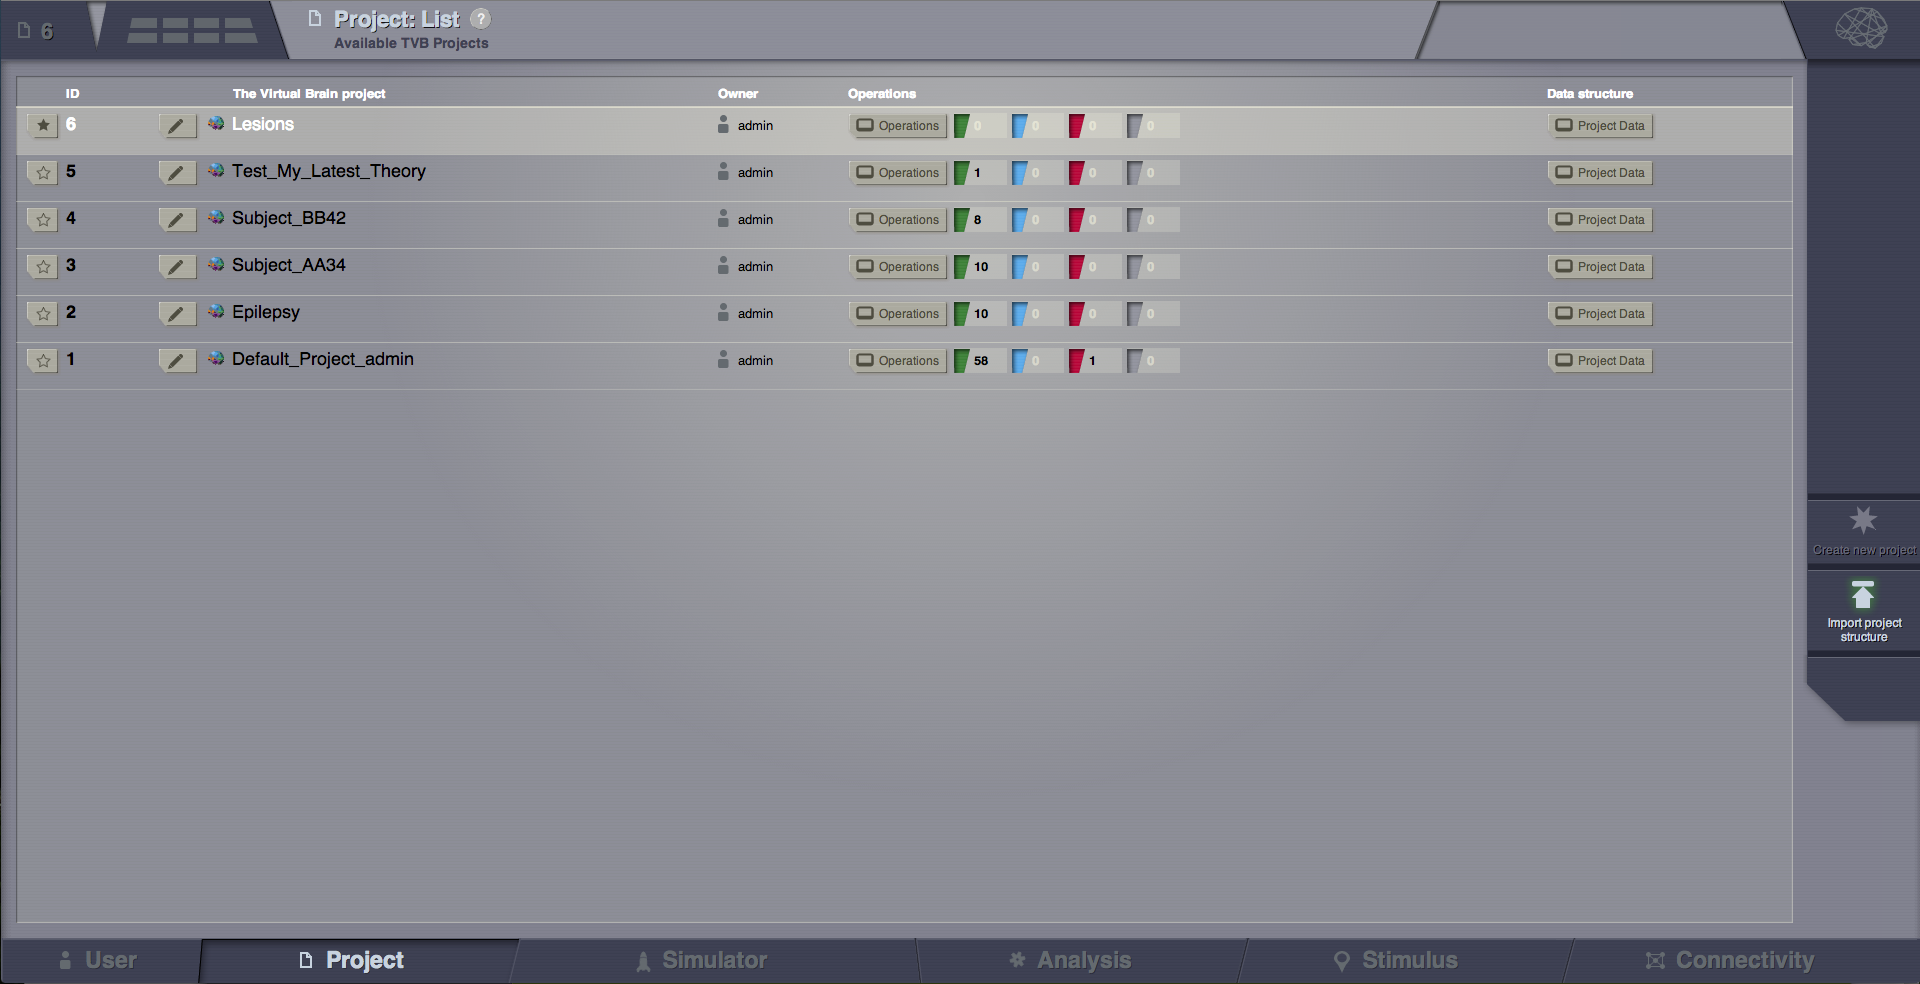
\includegraphics[width=0.47\textwidth]{images/ui_projects.png}}
    \\
    \subfloat[][]{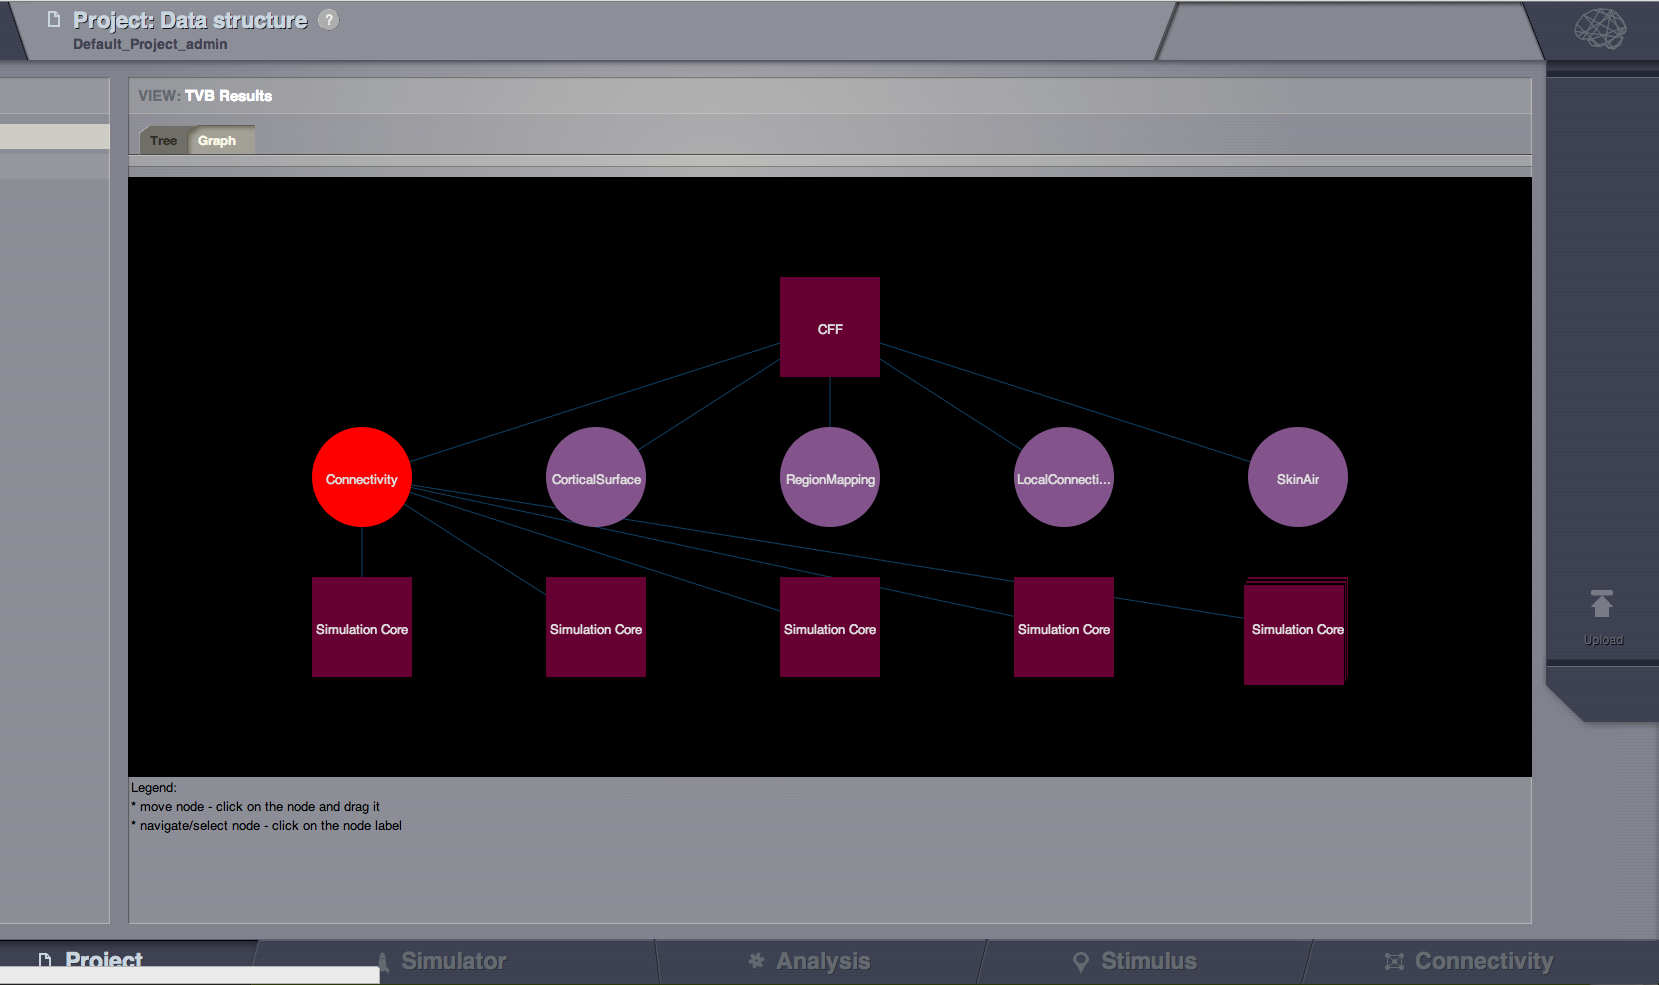
\includegraphics[width=0.47\textwidth]{images/ui_project_graph.png}}
    \\
    \subfloat[][]{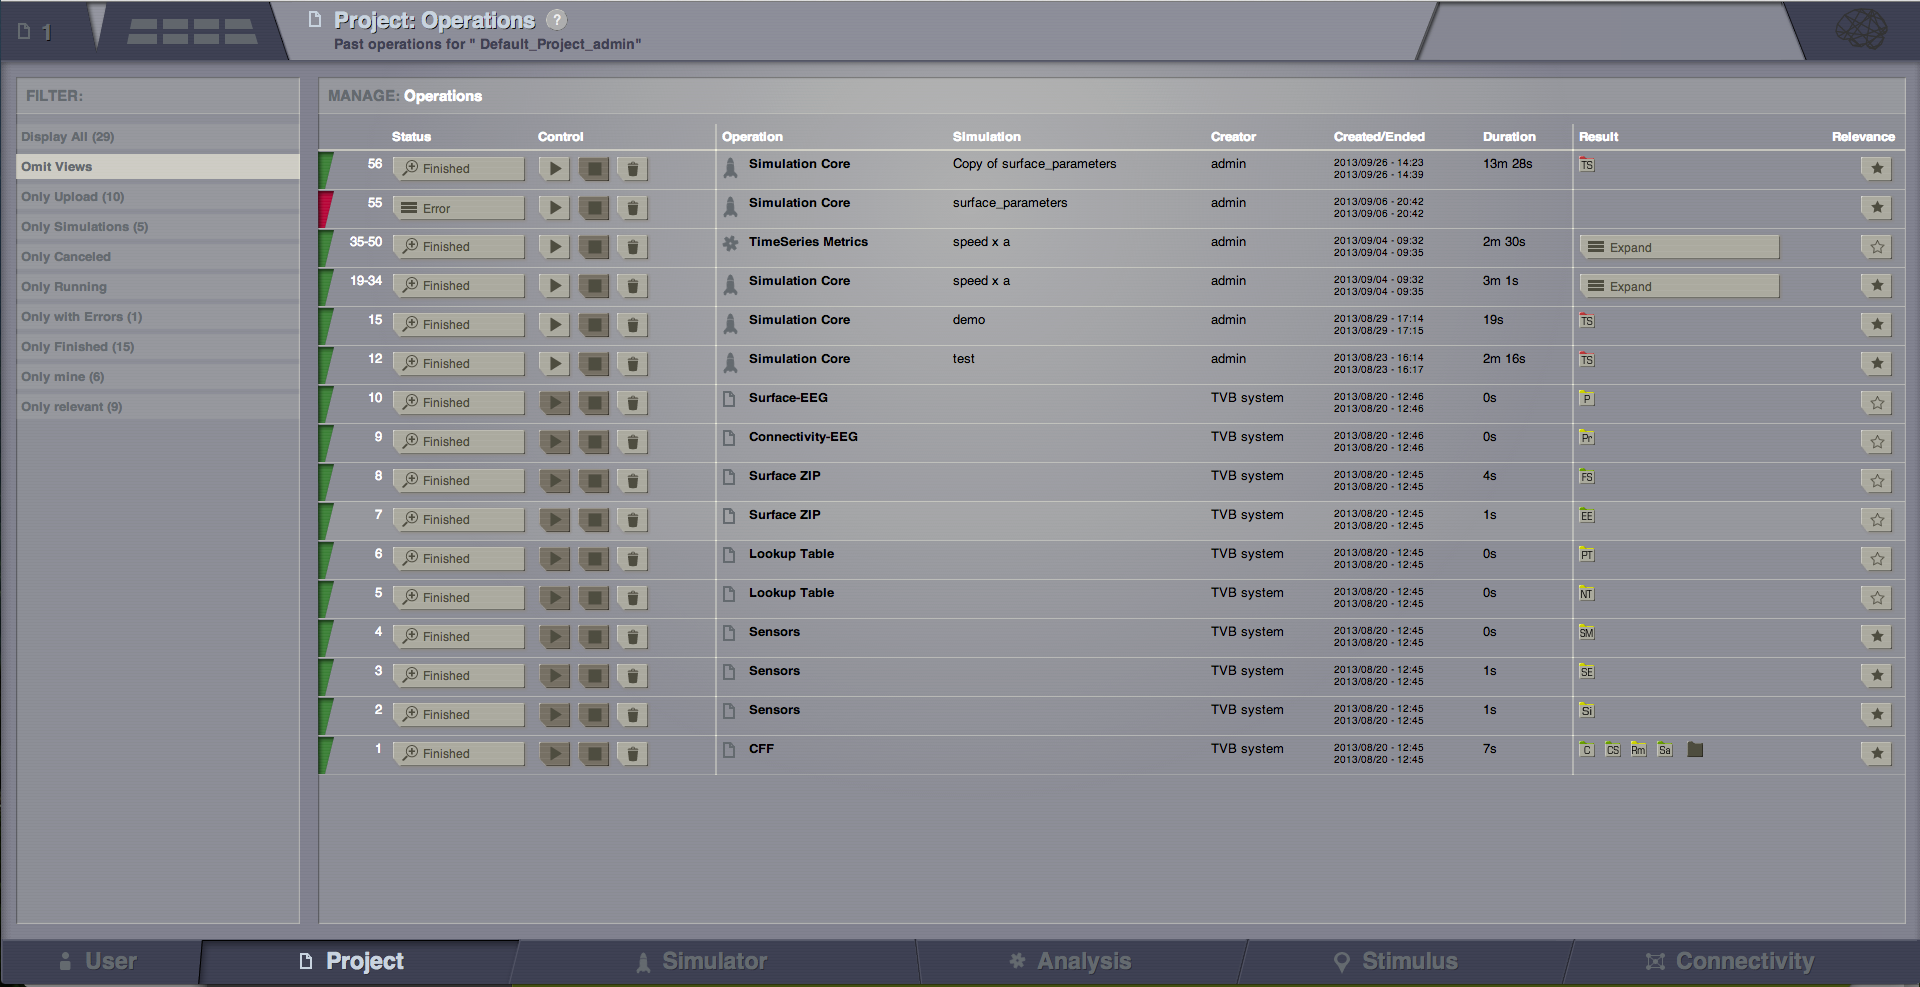
\includegraphics[width=0.47\textwidth]{images/ui_project_operations.png}}
    \\
    \subfloat[][]{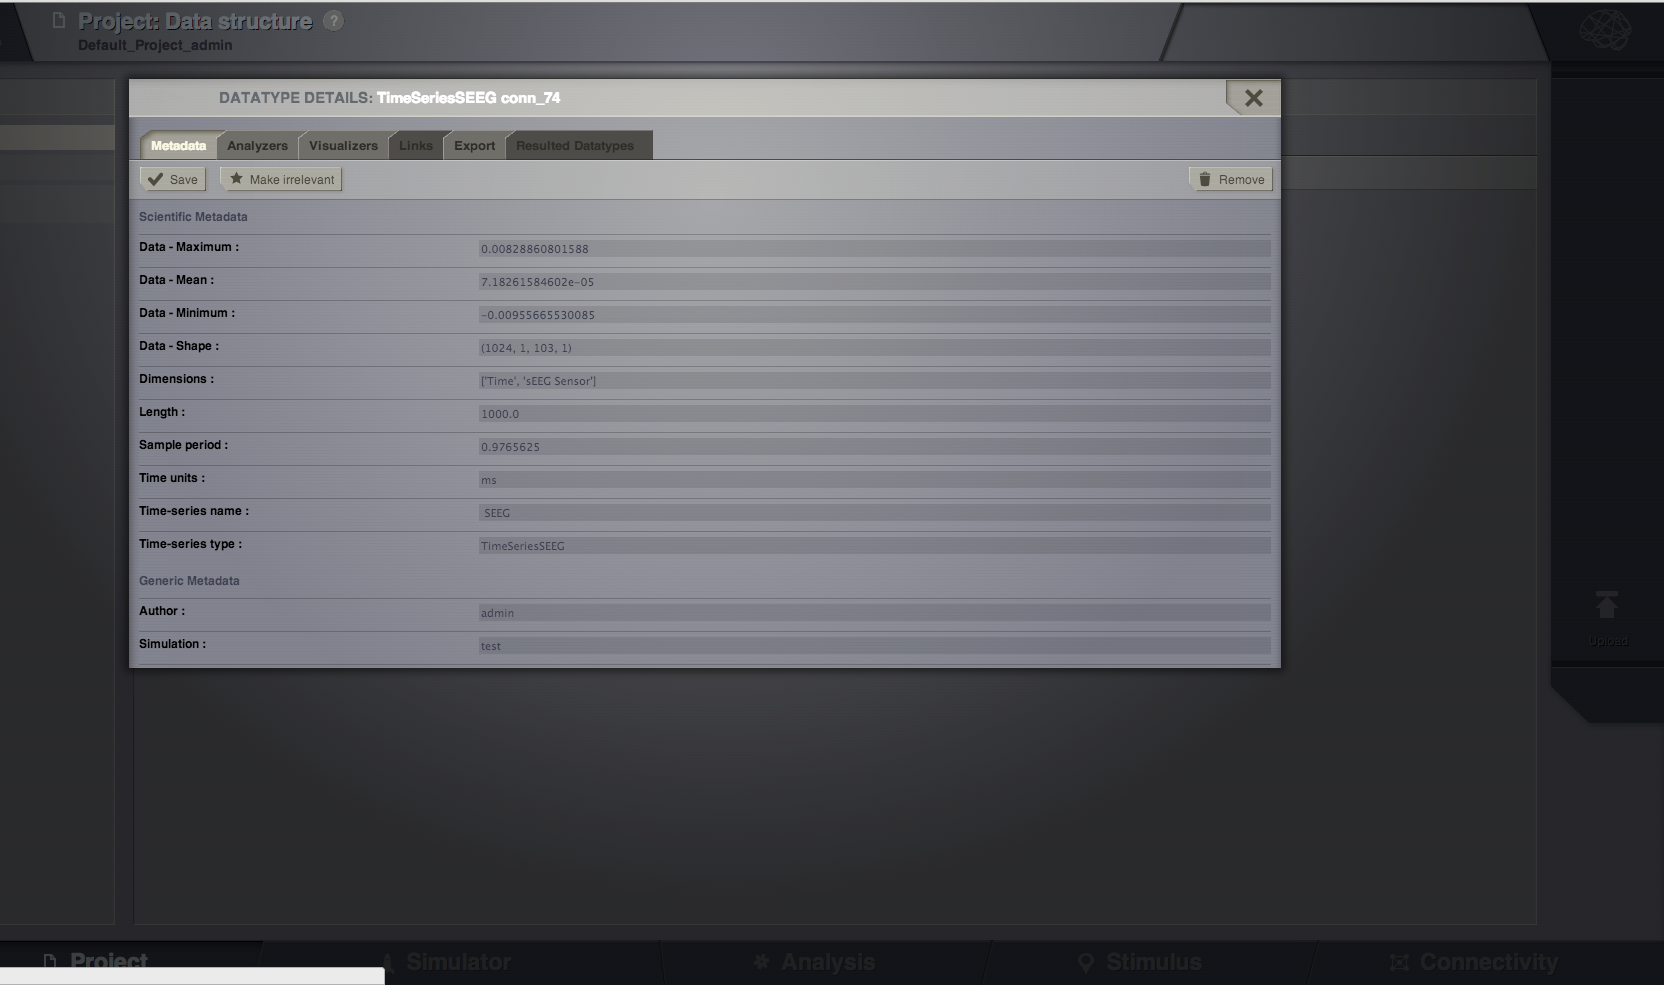
\includegraphics[width=0.47\textwidth]{images/ui_project_datatype_details.png}}
    \caption{\TVB Data Organization
    (A) View all Projects
    (B) 2D graph display of Operations with their input and output DataTypes 
    (C) View all Operations in current project with their status, duration, results, etc
    (D) DataType details and further available operations for it. This menu becomes available after clicking a DataType result from several places in \TVB }
        \label{fig:project}
\end{figure}

    An \emph{Account} or \emph{User} is needed for accessing \TVB through
    the web interface.  When \TVB web interface is fired for the first
    time, the G-User is requested to set his or her username and a
    password for the first account which acts under an
    \emph{administrator} role. Later on, more users can \emph{register}
    for other accounts, that should be previoulsy validated by the admin
    account.

    A \emph{Project} in \TVB is a logical grouping entity, which  can be
    used in several ways by the end-user;  for example one could choose to
    create a project for each experiment in \TVB, while others might
    create projects for each subject of a group. Each project has a single
    \emph{User} (or \emph{Account}) as owner, but a project can be shared
    with multiple users to allow for collaborative reasearch.

    Any execution of an Adapter results into an \emph{Operation} in the
    context of a project. Multiple operations will be executed under the
    same project. For example we will have operations created for each
    execution of a simulation, each run of a Fourier analyzer, or launch
    of a Brain Visualizer. An operation changes status over time, from
    \emph{started} into \emph{canceled}, \emph{finished successfully} or
    \emph{finished with error}. One operation can have multiple input and
    output parameters and parameters can be scalars or DataTypes.

    A \emph{Workflow} in \TVB is a set of operations with they artifacts,
    and wraps around a simulation as leading component. A workflow can be
    seen as a default \emph{tag} placed by the system on Operations and
    DataTypes  which are logically connected, as resulting one after the
    other. Custom tags can also be added by the end-user both on DataTypes
    and Operations, for tracking entities inside a Project.

    \subsubsection{Simulator Interface}
    
    \note[ld]{Fill description for this}
    
    \subsubsection{Analysis \& Visualizers}

\TVB does not aim to compete at the analysis level with other tools in
Neuroscience,  highly specialized and with great history in data
analysis, like  FSL or SPM.  What we offer is a minimalist set or
algorithms to post-process your  simulated results (or even process
imported patient measured scans) inside \TVB, mainly for quick
validations.

We have created inside \TVB adapters for \emph{Fast ICA} from the
python library \emph{sklearn},  we've implemented a python version of
\emph{Fourier Spectral Analysis},  we have even wrapped the Matlab
library \emph{BCT} \url{https://sites.google.com/site/bctnet/}, and
others as analyzers.

For each of the DataTypes produced in \TVB, one or multiple
visualizers are available.   \TVB has couple of  visualizer types,
each developed with the technology providing better support on the
specific requirements for the visualization in course:

 \begin{figure}[!htbp]
    \subfloat[][]{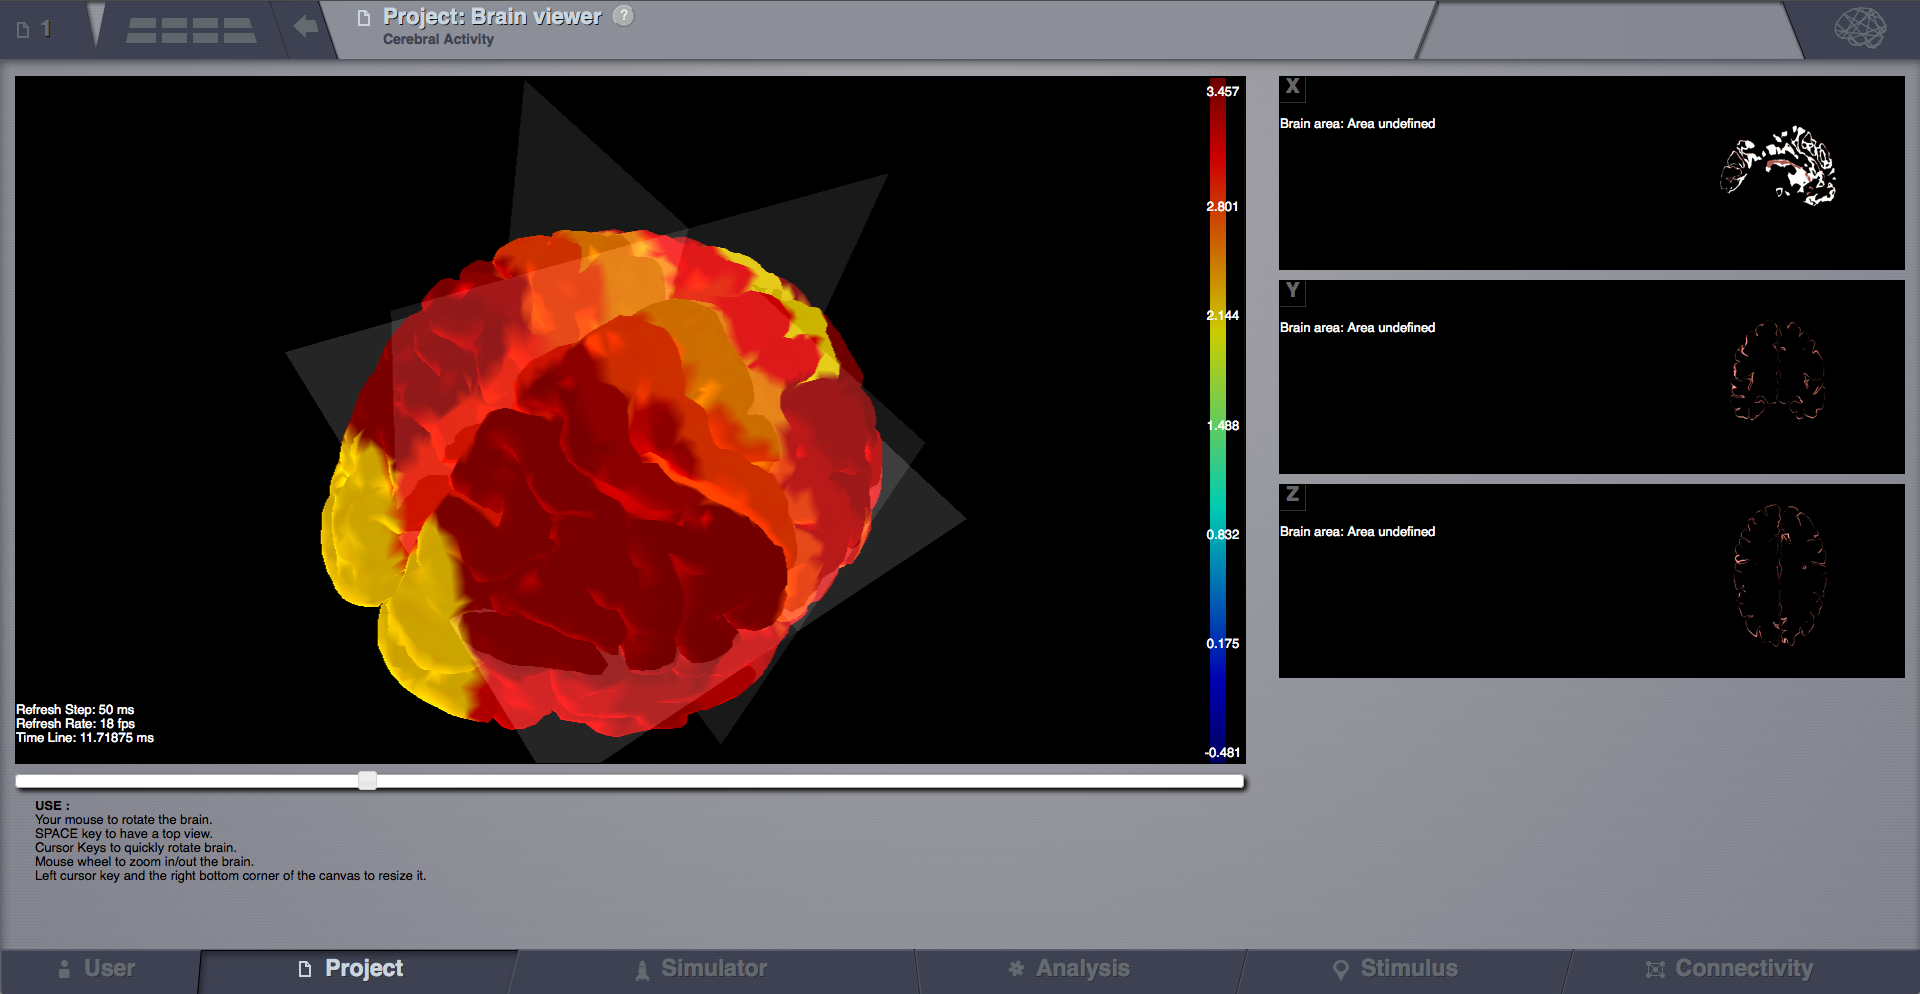
\includegraphics[width=0.48\textwidth]{images/ui_view_brain.png}}
    \\
    \subfloat[][]{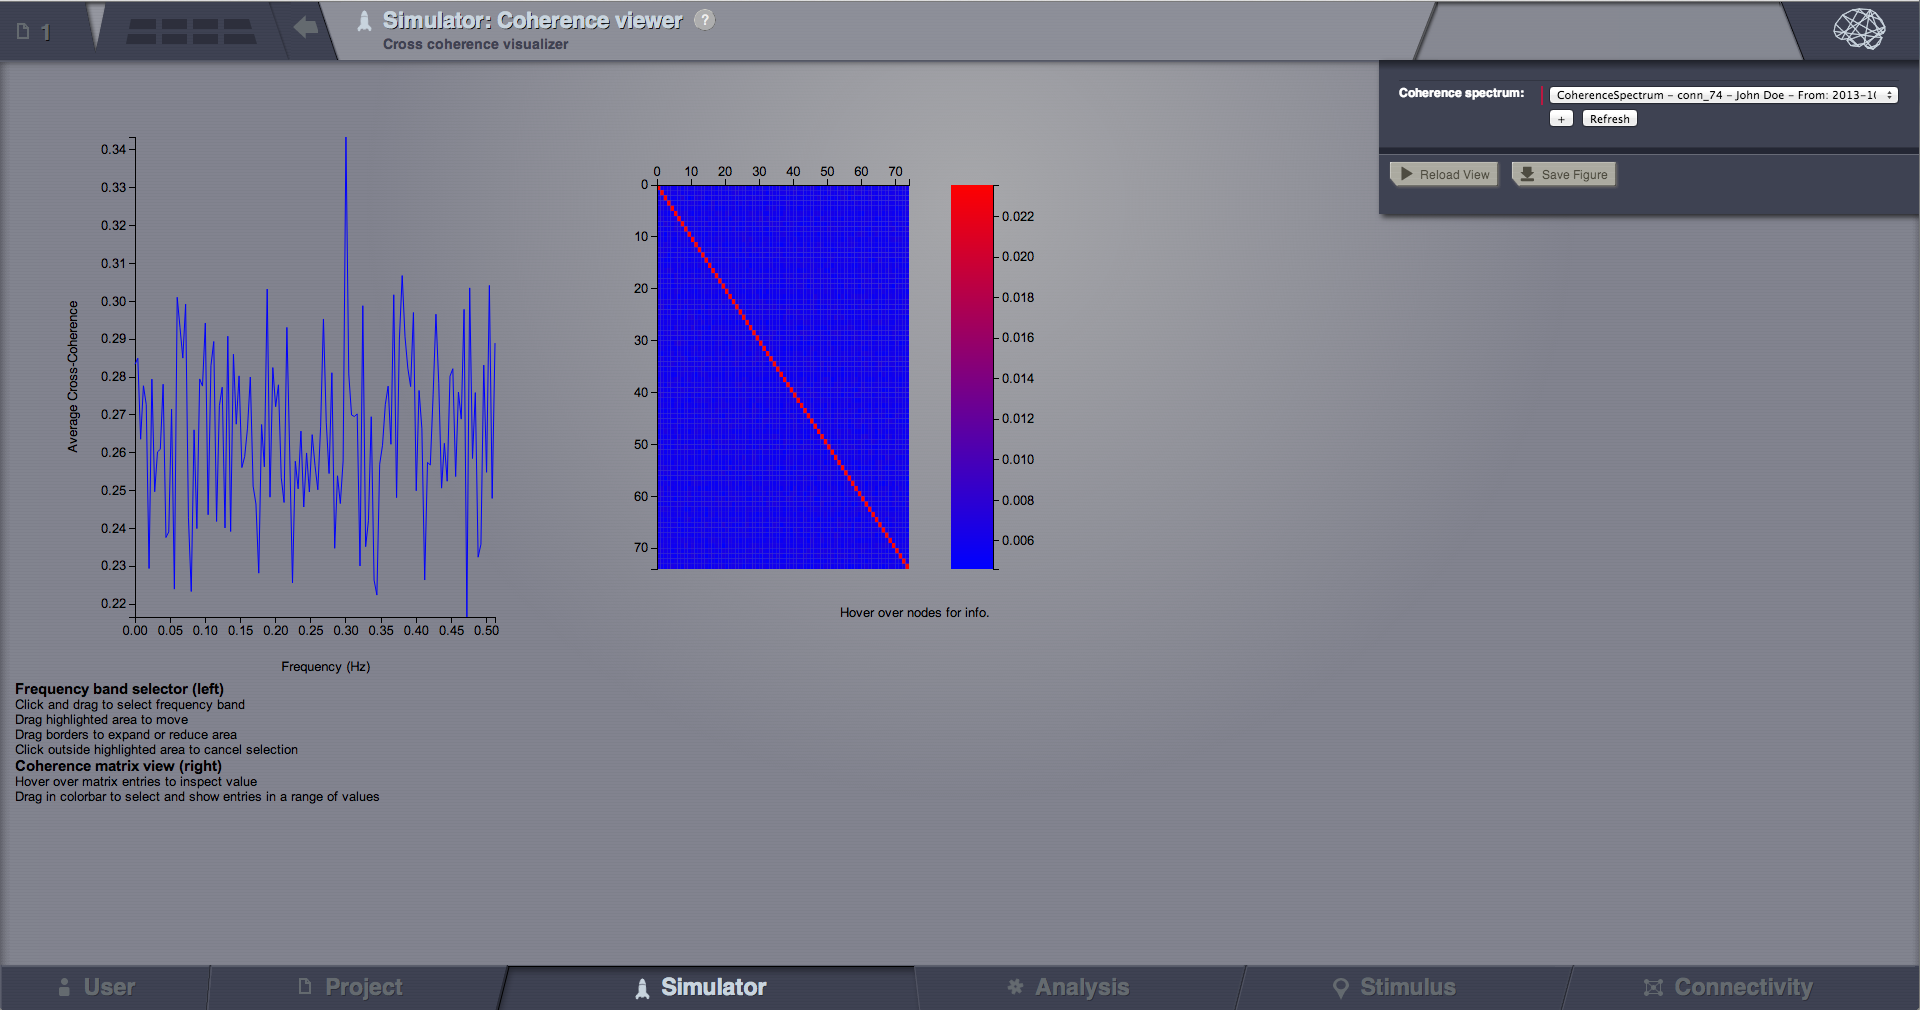
\includegraphics[width=0.48\textwidth]{images/ui_view_coherence.png}}
    \\
    \subfloat[][]{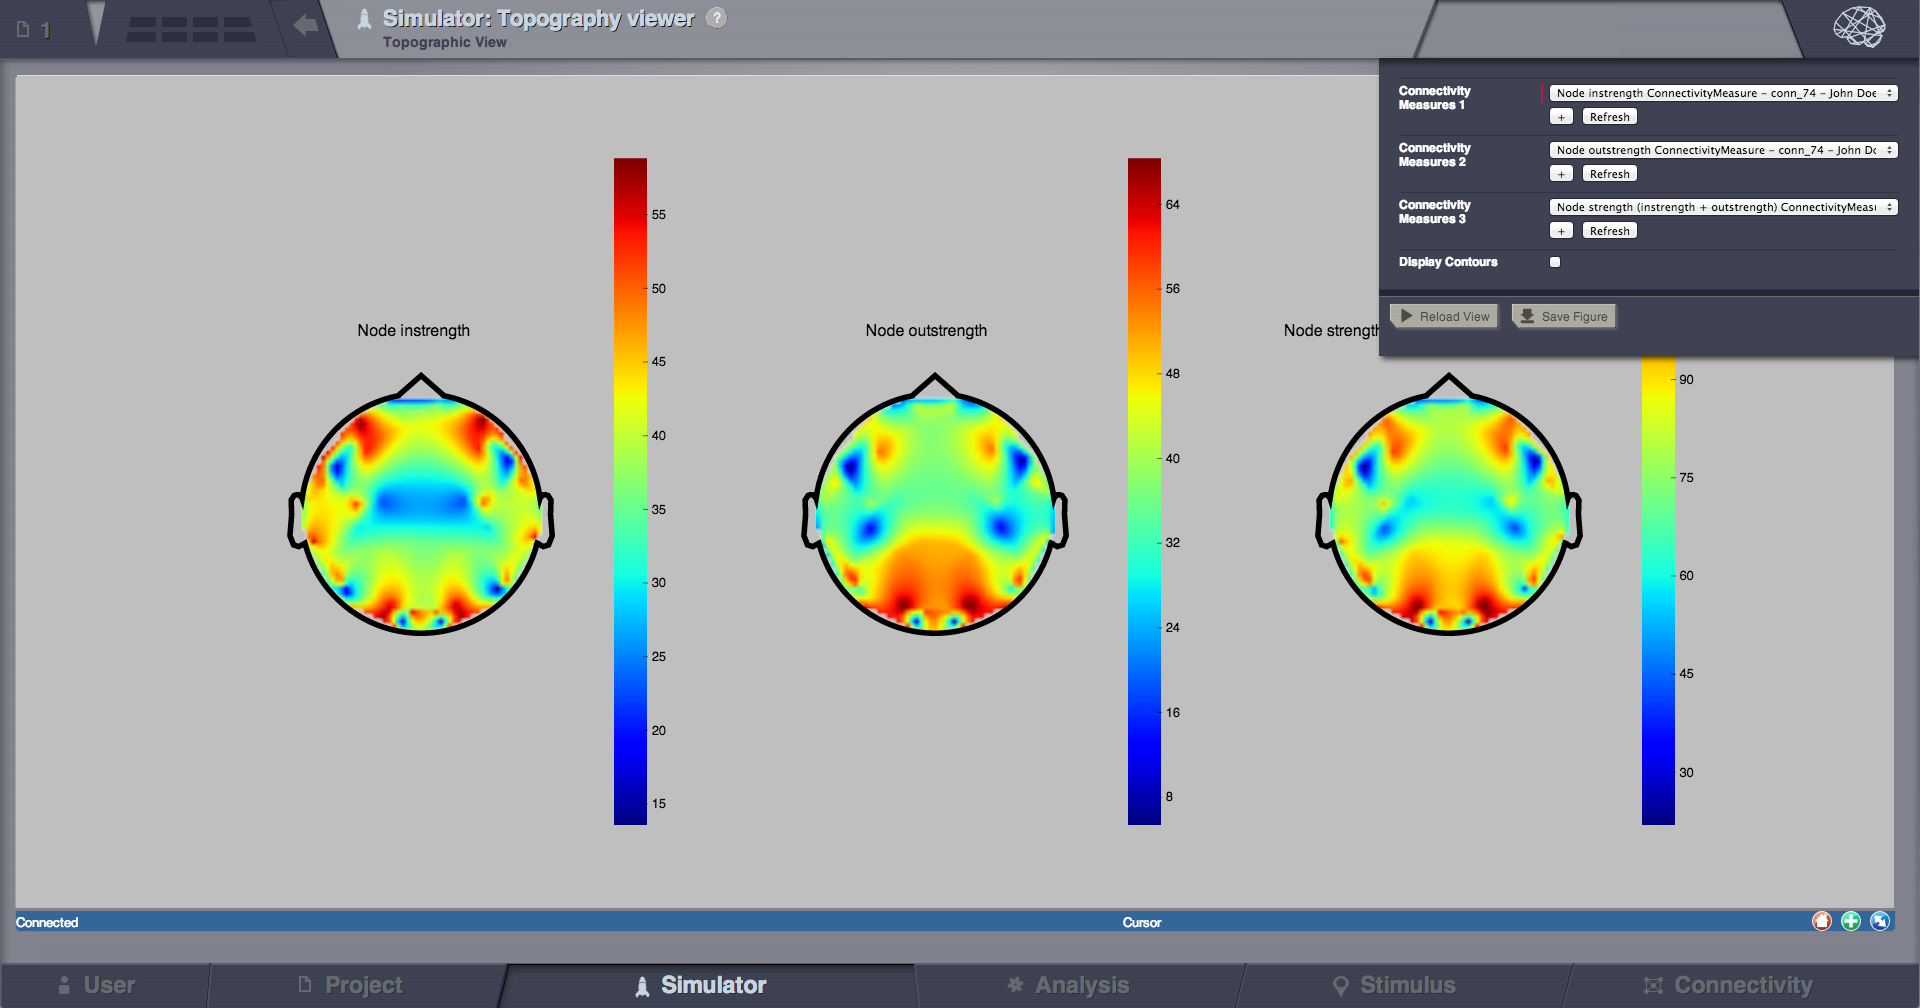
\includegraphics[width=0.48\textwidth]{images/ui_view_topo.png}}
    \\
    \subfloat[][]{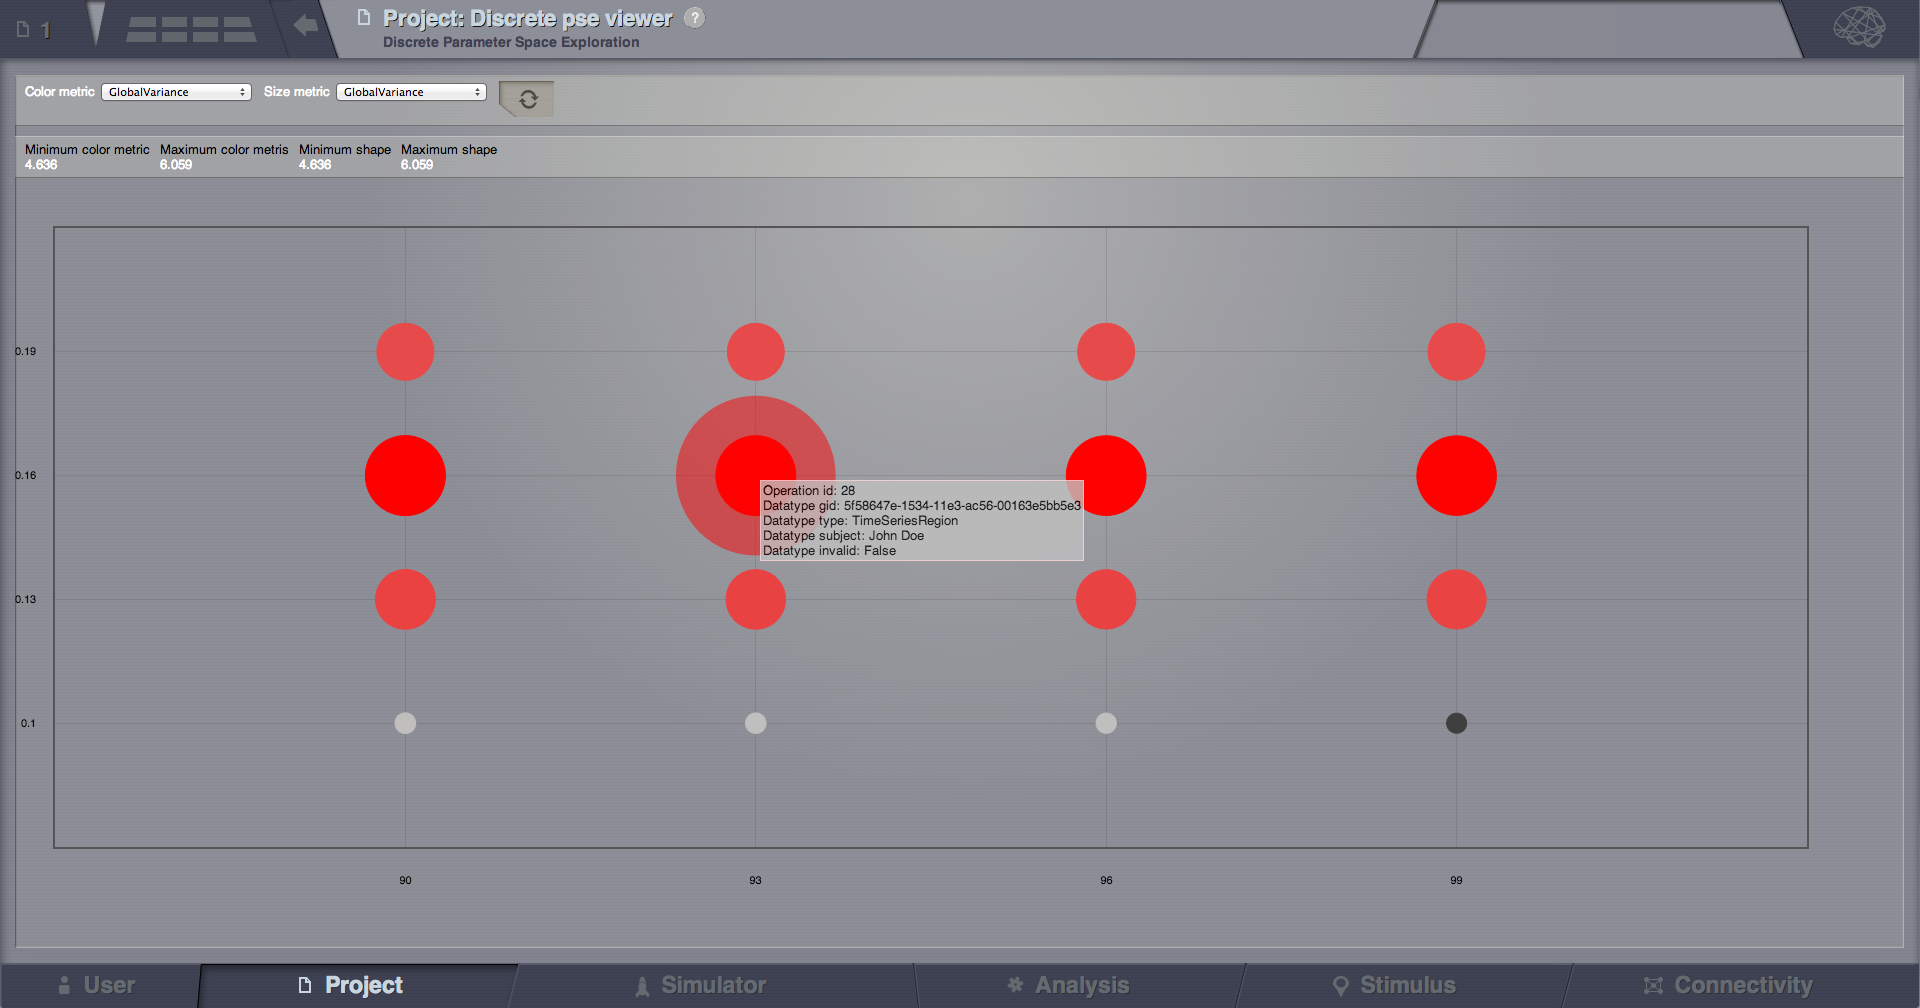
\includegraphics[width=0.48\textwidth]{images/ui_view_pse.png}}
    \caption{\TVB visualizers: 
    (A) WebGL: 3D display of region level simulated signal, mapped on a brain cortical surface
    (B) SVG: Cross Coherence
    (C) MPLH5:  Topograhic view with Connectivity in/out strength measures
    (D) FLOT: Parameter Space Exploration results grid}
        \label{fig:viewers}
\end{figure}

\begin{enumerate}

    \item \emph{WebGL viewers:} are based on \emph{HTML 5 Canvas} element
    and the \emph{gl} context. These viewers offer 3D nice display,
    vectorial zoom support, user interaction with the scene (rotate,
    translate), quick response (even when thousands of vertices and edges
    are to be manipulated) and good resolution for the images exported.
    
    \item \emph{SVG viewers:} offer great selection, zoom and scaling
    effects and extraordinary quality for the exported artifacts, while
    having a relatively low number of elements to display on the page. We
    use such viewers for manipulating and displaying TimeSeries,
    Covariance or Cross Coherence DataType results.

    \item \emph{MPLH5 viewers:}  emph{Matplotlib} has an \emph{HTML 5}
    backend that we use for viewing some of \TVB DataTypes (like
    Fourier or Wavelet) url{https://code.google.com/p/mplh5canvas/}

    \item \emph{Other} simpler viewers in \TVB are using JIT
    \url{http://philogb.github.io/jit/} or FLOT
    \url{http://www.flotcharts.org/} - JS libraries. These are mainly
    2D graph displayers for some simple \TVB generated data.

\end{enumerate}


\subsubsection{Connectivity Tool}

    \emph{Connectivity} in the context of \TVB is a DataType, mapping structural
    information about a subject (a real single individual or an average template). For
    editing and viewing a Connectivity, \TVB has a specific page, where
    the \emph{G-User} can manipulate connectivity strength and lengths
    starting from the granularity of an edge.

    We do not store or use information about the exact anatomical path or
    a connection, only the region centers and connection weights and
    lengths.

 \begin{figure}[!htbp]
    \centering
    \subfloat[][]{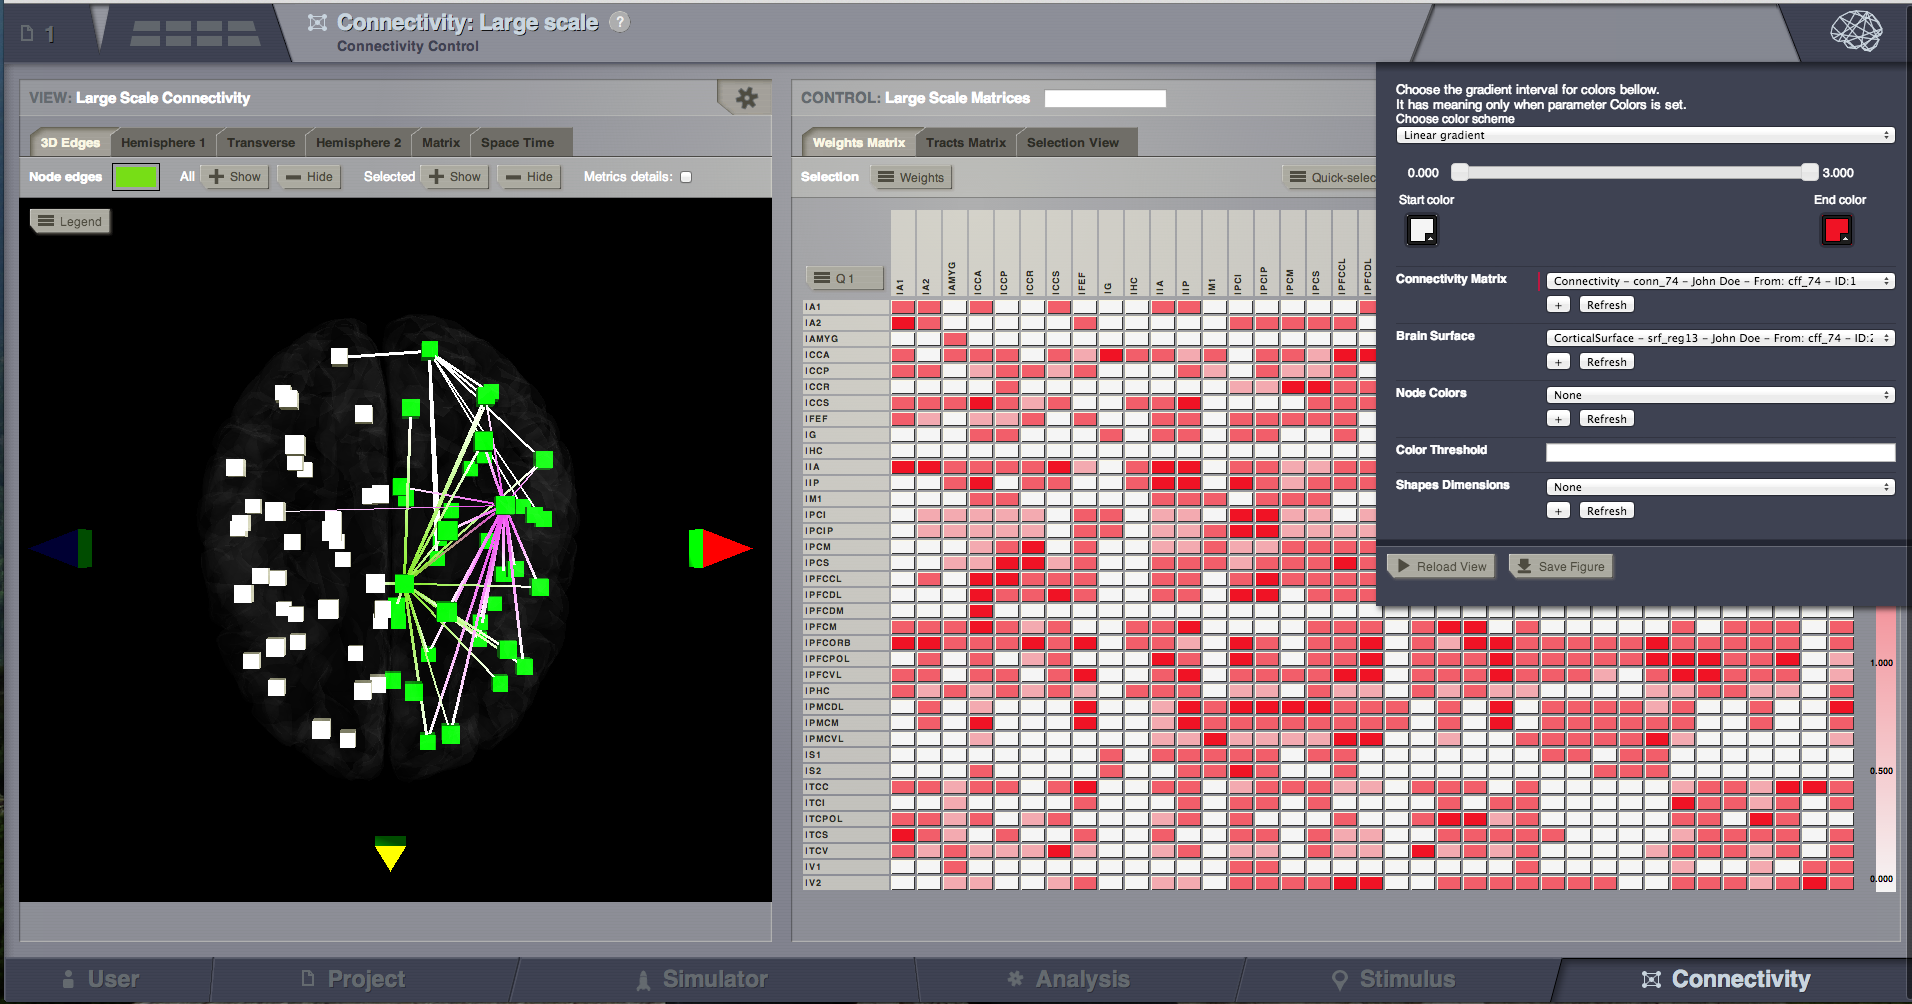
\includegraphics[width=0.48\textwidth]{images/ui_connectivity.png}}
    \\
    \subfloat[][]{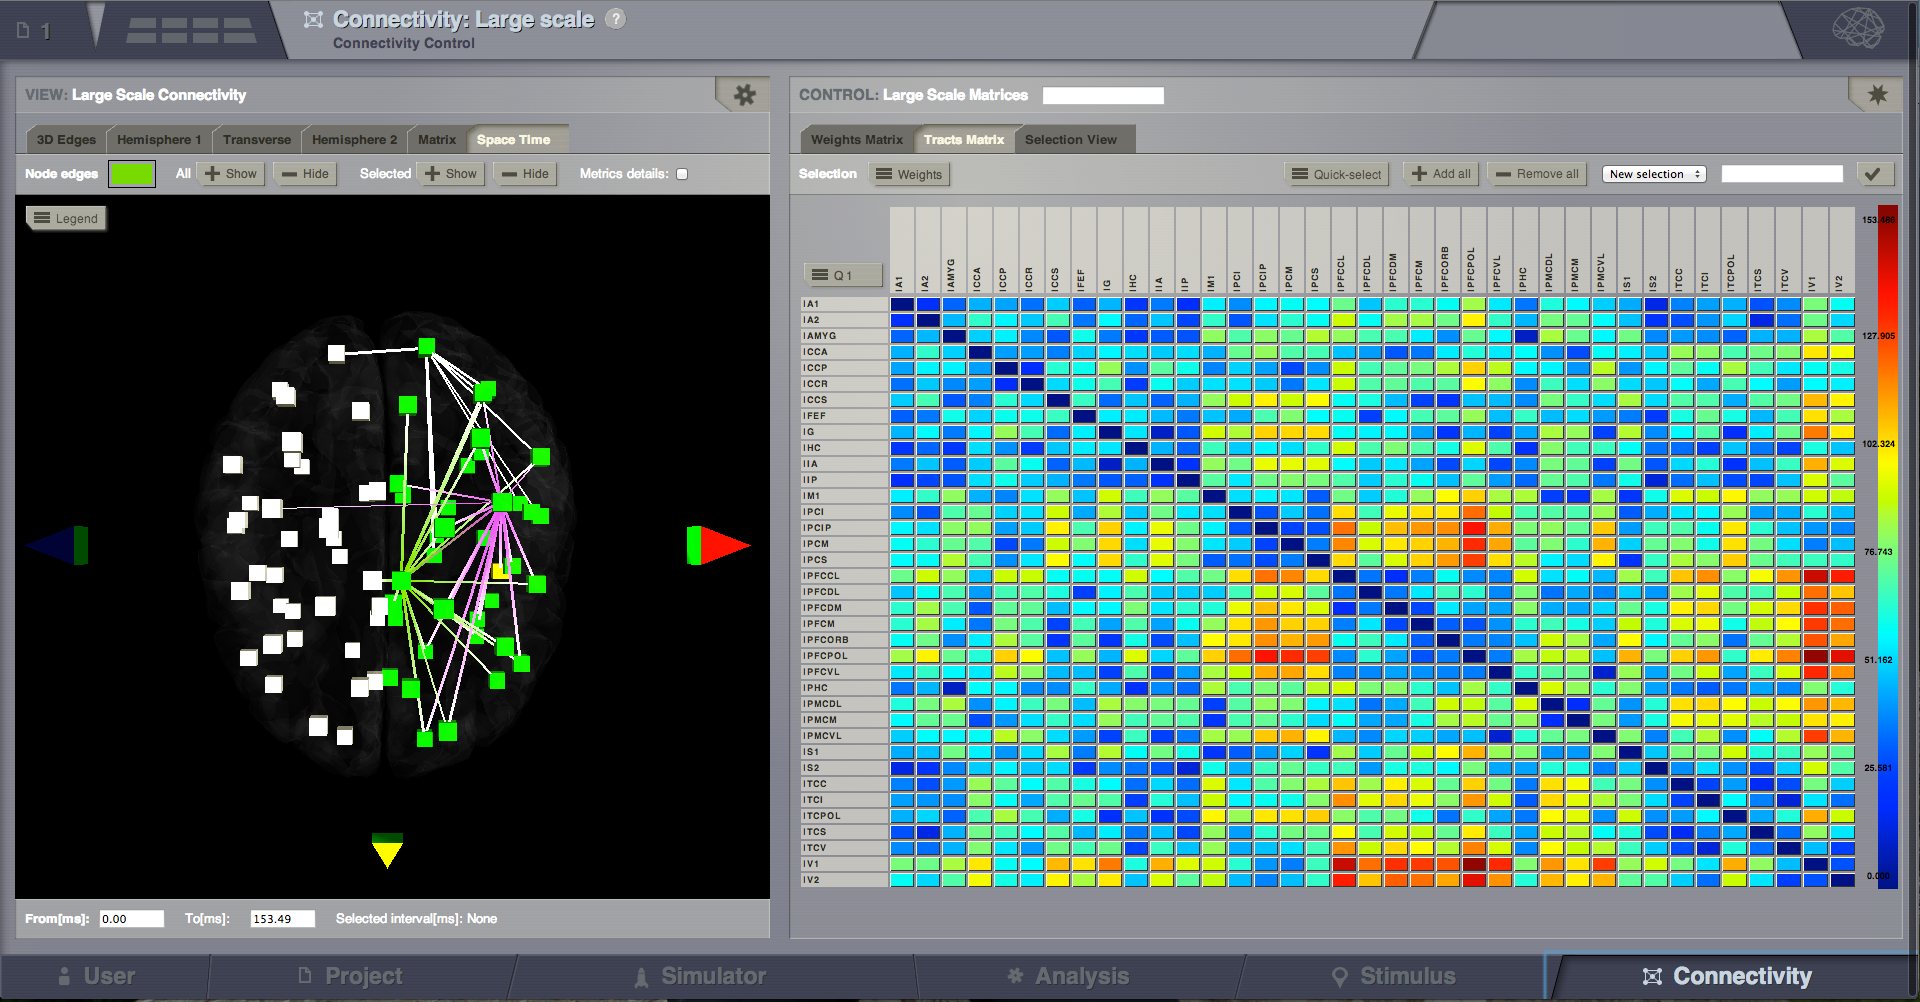
\includegraphics[width=0.48\textwidth]{images/ui_connectivity_delays.png}}
    \caption{Connectivity Tools: 
    (A) Left side: Displaying weighted connections between selection of nodes, with 3D manipulation.
    Right side: Editing weight connections, singular or bulk.
    (B) Left side: Show effect of connectivity delays (in milliseconds) when conductions speed is 1 mm/ms.
    Right side: Editing and displaying one quadrant from the matrix of connection tracts.}
        \label{fig:connectivity}
\end{figure}



\subsection{Python Scripting}

\texttt{hello\_brain.py}
To give a basic feel for scripting \TVB simulations, we will 
walk through a simple example of a region-level simulation. We 
start with

\begin{lstlisting}
from tvb.simulator.lab import *
\end{lstlisting}

\noindent which is an all-in-one module making writing scripts
shorter, in the style of \texttt{pylab}, as it imports everything
from \texttt{pylab}, \texttt{numpy} and most of \TVB's simulator
modules. Next, we build a simulator object:

\begin{lstlisting}
sim = simulator.Simulator(
    model        = models.Generic2dOscillator(), 
    connectivity = connectivity.Connectivity(),
    coupling     = coupling.Linear(a=1e-2),
    integrator   = integrators.HeunDeterministic(),
    monitors     = (
        monitors.TemporalAverage(), 
    )
)
\end{lstlisting}

\noindent where we've employed a two dimensional oscillator
with default parameters, the default connectivity, a linear 
coupling function with a slope of $1e-2$, and deterministic
Heun integrator and a monitor that temporally averages the 
network dynamics before providing output.

While \TVB strives to keep modules independent of one another,
it is typical for mathematical dependencies to arise between, 
for example, the mass model and the integration time step, so
after configuring a simulator object, it is necessary to invoke

\begin{lstlisting}
sim.configure()
\end{lstlisting}

which results in walking the tree of objects, checking and 
configuring the constraints among parameters recursively.

The next step is to run through the simulation, collecting
output from the simulator. In this case, it is as simple as
\begin{lstlisting}
ys = array([y for ((t, y),) 
          in  sim(simulation_length=3e2)])
\end{lstlisting}
\noindent where the simulator has been called, returning a 
generator which performs the integration and returns, for each
monitor, the current time and activity. In a case where EEG 
and fMRI monitors, for example, were used, we might write
\begin{lstlisting}
eeg, mri = [], []
for (t_eeg, y_eeg), (t_mri, y_mri) in sim(3e2):
    if y_eeg is not None:
    eeg.append(y_eeg)
    ...
\end{lstlisting}
\noindent Because fMRI and EEG monitors have very different
timescales, whenever one monitor return data and the others do
not, the others contain \texttt{None}, hence the check. Building
more complex logic in this loop would permit, for example, online
feedback and modification of connectivity. 

After the simulation loop has finished, you may wish to see the
result, following the previous listing, 
\begin{lstlisting}
plot(ys[:, 0, :, 0], 'k', alpha=0.1)
\end{lstlisting}
\noindent Here we note that \texttt{ys} is four dimensional. The 
simulator has the convention of treating  mass model state as a
three dimensional array of state variables by nodes by statistical
modes. Because \texttt{ys} is an array collected over time, the first
dimension is time, and the plot here is of each node's first state
variable, over time.

Many more demonstrations of the various features of the simulator
can been found in scripts distributed with the sources of \TVB, or 
browsed online at \url{https://github.com/the-virtual-brain/scientific_library/tree/trunk/tvb/simulator/demos}.
In the next section, we will go into detail about the different
components of the simulator.

\subsection{MATLAB Scripting}

Due to the popularity of MATLAB in the neuroscience community, an
interface from MATLAB to \TVB has been introduced that allows a MATLAB
script to design a TVB simulation, run it on TVB and retrieve the 
results. The MATLAB toolbox is provided separately from TVB, at
\url{https://github.com/the-virtual-brain/matlab-tvb}.
In the following, we give a short demonstration and 
describe implementation and rationale.

Because the MATLAB functions need to know the address of the server,
so we take any of the URLs used by the Web UI (here, the one provided
when launching TVB):

\begin{lstlisting}
sv = vb_url('http://127.0.0.1:8080/user/')
\end{lstlisting}

To run simulations without blocking MATLAB, a multiprocessing Pool
is used. We reset the pool and change the number of processes to 6

\begin{lstlisting}
vb_reset(sv, 6)
\end{lstlisting}

Next, we can query the server for information on the classes available,
and also get help for each of the classes

\begin{lstlisting}
info = vb_dir(sv);
\end{lstlisting}

\noindent where info is a cell array of structs, one per module (models,
monitors, etc.) and each struct has a field per class (models.JansenRit, 
models.Kuramoto, etc.). Each of these fields contains the details on 
the class, including all the parameters that can be set. 

To build a simulation, we start with an empty struct
and fill in the details for each part

\begin{lstlisting}
sim = [];

sim.tf = 1e3 % simulation length milliseconds
sim.model.class = vb.models.Generic2dOscillator;
sim.model.a = -2.1;

sim.connectivity.class = 'Connectivity';
sim.connectivity.speed = 4.0;

sim.coupling.class = 'Linear';
sim.coupling.a = 0.002;

sim.integrator.class = 'HeunDeterministic';
sim.integrator.dt = 1e-2;
\end{lstlisting}

Monitors are specified similarly but as a cell array there may be
several of them:

\begin{lstlisting}
sim.monitors{1}.class = 'TemporalAverage';

sim.monitors{2}.class = 'Raw';
sim.monitors{2}.period = 1.0; % ms
\end{lstlisting}

Lastly, we submit the struct as a new simulation

\begin{lstlisting}
[id, data] = vb_new(sv, sim);
\end{lstlisting}

\noindent Lastly, results are returned in a struct, here named data
where each field contians the output of a monitor and can be plotted
and analyzed as a regular MATLAB dataset:

\begin{lstlisting}
plot(data.mon_0_TemporalAverage.ts,...
     squeeze(data.mon_0_TemporalAverage.ys)')
\end{lstlisting}

The implementation of this interface is a combination of an additional
CherryPy controller providing an HTTP/JSON API, running on the same 
server as the Web UI, and a set of MATLAB functions that send HTTP 
GET requests to the server. An implementation based on MEX functions 
invoking the Python library directly was considered, for reasons of 
performance, however, it was judged that such an implementation may be
difficult to stabilize and maintain, given that it would require binary
compatibility between MATLAB, Python and the C compiler. Two additional 
advantages of an HTTP API are that most computational environments have
the ability to connect and make HTTP requests, allowing other programs 
like Perl or Mathematica take advantage of TVB and the approach naturally
extends to work over the network, should TVB be running on another machine.





